%\documentclass[11pt,respuestas,a4]{aleph-examen}
\documentclass[11pt,a4]{aleph-examen}
% Se puede ver la documentación aquí: 
% https://github.com/alephsub0/LaTeX_aleph-examen

% -- Paquetes adicionales 
\usepackage{aleph-comandos}
\usepackage{booktabs}
\usepackage{multicol}
\usepackage{pgfplots}

% -- Datos 
\institucion{Escuela de Ciencias Físicas y Matemática}
\carrera{Medicina Veterinaria}
\asignatura{Matemática I*}
\tema{Taller no. 1}
\autor{Fernando Jiménez T.}
\fecha{Semestre 2024-2}


\logouno[0.14\textwidth]{Logos/logoPUCE_04_ac}
\definecolor{colortext}{HTML}{0030A1}
\definecolor{colordef}{HTML}{0030A1}
\fuente{montserrat}


\begin{document}

\encabezado

\section*{Indicaciones}
\begin{itemize}[leftmargin=*]
\item 
    En esta actividad se evalúa si el estudiante \textit{(Criterio 1.1) comprende los conceptos fundamentales de lógica matemática, teoría de conjuntos y números reales aplicables en su campo.}
\item 
    El taller se desarrollará de manera colaborativa en grupos de trabajo asignados por el docente.
\item 
    Se permitirá el uso de libros de texto y notas de clase.
\item 
    Cada grupo deberá resolver los problemas propuestos y justificar cada solución de manera clara, indicando los procedimientos utilizados y los conceptos aplicados.
\item 
    Al final del taller, cada grupo presentará sus resultados y explicará sus razonamientos al resto de la clase, mediante una exposición.
\end{itemize}

\section*{Ejercicios}

\begin{preguntas}

%%%%%%%%%%%%%%%%%%%%%%%%%%%%%%%%%%%%
\item 
    Un veterinario está monitoreando la frecuencia cardíaca de un gato. La frecuencia cardíaca normal para un gato es de entre 140 y 220 latidos por minuto. La frecuencia cardíaca se puede formular como la función $f$ definida por la regla:
    \begin{center}
    	«Dividir el número de latidos por el tiempo medido en minutos».
    \end{center}
    Por simplicidad, el veterinario suele contar la cantidad de latidos en 15 segundos.
% ---------------------------
    \begin{enumerate}[label=\textit{\alph*)}]
    \item 
        Escribir la función $f(x)$ que representa la frecuencia cardíaca de un gato, donde $x$ representa la cantidad de latidos que se cuenta en 15 segundos. 
    \item 
        Un gato llega con el veterinario y para poder ingresarlo debe medir su frecuencia cardíaca. Después de 15 segundos, el veterinario ha contado 30 latidos. Determinar la frecuencia cardíaca del gato y verificar si está dentro del rango normal.
    \item 
        Identificar el tipo de función que es $f$ y realizar una gráfica de la función. \textit{Sugerencia}: Para graficar la función, hacer la tabla de valores con los puntos $x$ del conjunto $\{50,100,150,200,250\}$.
    \item 
        Identificar el dominio y recorrido de la función $f$. Explicar su respuesta.
    \item 
        Se conoce que la frecuencia cardíaca normal de un gato está dentro del intervalo $[140,220]$. Determinar el conjunto de todos los puntos del domino de $f$ cuya imagen está dentro del intervalo $[140,220]$.
    \item 
        Dar dos conclusiones del análisis realizado en los literales anteriores.
    \end{enumerate}
% ---------------------------
\begin{respuesta}
\begin{enumerate}[label=\textit{\alph*)}]
    \item
        La función se puede definir como:
        \[
            f(x) = \frac{x}{15} \cdot (60) = 4x.
        \]
    
    \item 
        Para calcular la frecuencia cardíaca con 30 latidos, sustituimos $x$ por $30$ en la función $f$, es decir,
        \[
            f(30) = 4(30) = 120.
        \]
        Como el gato tiene una frecuencia cardíaca de $120<140$, podemos concluir que no está dentro del rango normal.
    
    \item 
        La función $f$ es una función lineal. Una representación gráfica de esta función es:
        \begin{center}
        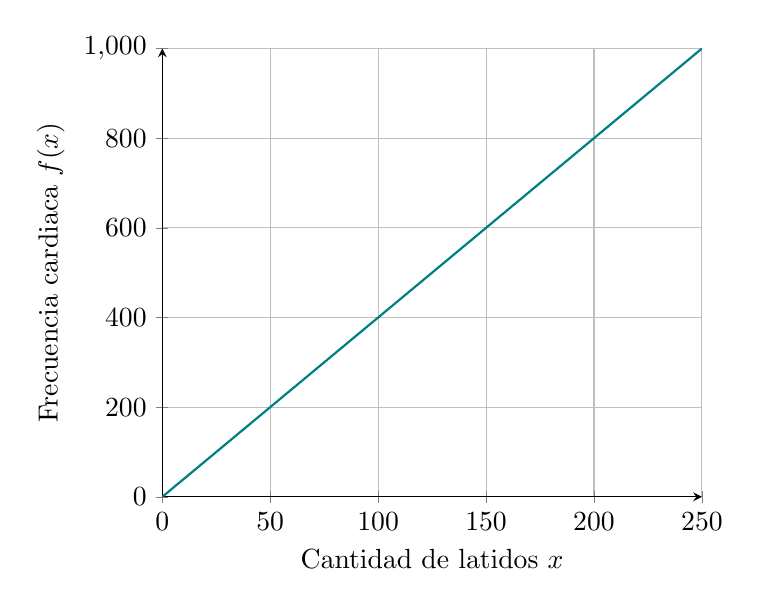
\begin{tikzpicture}
            \begin{axis}[
                axis lines = left,
                xlabel = {Cantidad de latidos $x$},
                ylabel = {Frecuencia cardiaca $f(x)$},
                ymin=0, ymax=1000, xmin=0, xmax=250,
                grid=both,
                domain=0:250,
                samples=100
            ]
            \addplot[color=teal, thick]{4*x};
            \end{axis}
        \end{tikzpicture}
        \end{center}
    
    \item 
        El dominio de la función es $\dom(f) = \R_+$ y el recorrido o imagen de $f$ es $\Img(f) = \R_+$.
    
        Tanto el dominio como el recorrido no pueden ser números negativos o el cero, pues un gato no puede tener $0$ latidos o un número negativo de estos. De igual forma, como $x > 0$, entonces $f(x) = 4x > 0$. 
    
    \item 
        Notemos que $140$ y $220$ son los extremos del intervalo. Como es una función lineal, basta con conocer los valores de $x$ para los cuales se obtiene una imagen de 140 y 220. Gráficamente, podemos notar que con $x = 35$ se obtiene que $f(35) = 140$ y con $x = 55$ obtenemos $f(55) = 220$. Por lo tanto, para cualquier punto $x \in [35,55]$ se tiene que $f(x) \in [140,220]$.\qedhere
\end{enumerate}
\end{respuesta}

%%%%%%%%%%%%%%%%%%%%%%%%%%%%%%%%%%%%
\item 
    Un veterinario calcula los costos de atención para los perros que llegan a su consultorio. El costo total (en dólares americanos) se puede expresar como la función:
    \[
        g(x) = 3x^2 + 12x,
    \]
    donde $x$ es el tiempo, medido en horas, que dura la consulta de un perro.
    % ---------------------------
    \begin{enumerate}[label=\textit{\alph*)}]
    \item 
        Factorizar la expresión del costo total.
    \item 
        Determinar el dominio de la función. Justificar su respuesta.
    \item 
        Graficar la función para el dominio calculado.
    \item 
        Un perro llega a su consultorio y tarde 2 horas y media en atenderlo. Calcular el costo de la consulta.
    \item 
        Analizando los literales anteriores, dar dos conclusiones sobre los resultados obtenidos.
    \end{enumerate}
% ---------------------------
\begin{respuesta}
\begin{enumerate}[label=\textit{\alph*)}]
	\item 
        Notemos que los factores en com\'un del binomio son $3x$, es decir, tenemos que:
    	\[
    	   3x^2 + 12x = 3x(x+4).
    	\]
    	Cada uno de los factores encontrados son polinomios de orden 1 y no es posible factorarlos más.
    	
    \item 
        Observemos que el tiempo solo puede ser un valor no negativo. Por lo tanto, el dominio de la función ser\'ia $\R_{\geq 0}$.
	
    \item 
        El gráfico de la función es:
        \begin{center}
        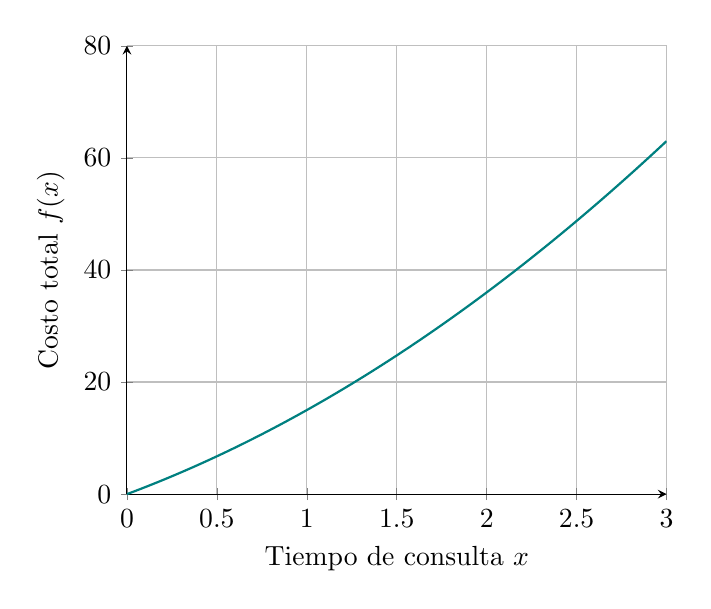
\begin{tikzpicture}
            \begin{axis}[
                axis lines = left,
                xlabel = {Tiempo de consulta $x$},
                ylabel = {Costo total $f(x)$},
                ymin=0, ymax=80, xmin=0, xmax=3,
                grid=both,
                domain=0:3,
                samples=100
            ]
            \addplot[color=teal, thick]{3*x^2 + 12*x};
            \end{axis}
        \end{tikzpicture}
        \end{center}
    
	\item 
        Para calcular el costo de la consulta, debemos evaluar la función $g$ en $x = 2.5$. Es decir,
    	\[
    	   g(2.5) = 3(2.5) (2.5+4) = 7.5(6.5) = 48,75.\qedhere
    	\]
\end{enumerate}
\end{respuesta}

%%%%%%%%%%%%%%%%%%%%%%%%%%%%%%%%%%
\end{preguntas}

\end{document}